\documentclass[12pt]{article}
\usepackage{graphicx}
\usepackage[ruled]{algorithm2e}
\usepackage{amsmath}
\usepackage{mathtools}
\usepackage{float}
\usepackage{booktabs}
\usepackage{pbox}
\usepackage{afterpage}
\usepackage{caption}
\usepackage{algorithmic}
\usepackage{lipsum}
\usepackage{titlesec}

\setcounter{secnumdepth}{4}

\titleformat{\paragraph}
{\normalfont\normalsize\bfseries}{\theparagraph}{1em}{}
\titlespacing*{\paragraph}
{0pt}{3.25ex plus 1ex minus .2ex}{1.5ex plus .2ex}


\renewcommand{\algorithmcfname}{ALGORITHM}
\SetAlFnt{\small}
\SetAlCapFnt{\small}
\SetAlCapNameFnt{\small}
\SetAlCapHSkip{0pt}
\IncMargin{-\parindent}


\hyphenation{op-tical net-works semi-conduc-tor}

\begin{document}
%
% paper title
% can use linebreaks \\ within to get better formatting as desired
\title{Smart Food Dispenser for Dogs}

\author{Pedro Anibarro$^1$\thanks{panibarro1@email.suagm.edu}
\and
Harry Miranda$^2$\thanks{hmiranda12@email.suagm.edu}
\footnotemark[1]}

\date{
    $^1$$^,$$^2$Department of Computer \& Electrical Engineering,\\
    Universidad del Turabo, Gurabo PR
}


% % make the title area
\maketitle

% ------------------------------------------------ Abstract ------------------------------------

\begin{abstract}
%\boldmath

Many dog owners do not feed their dogs in the correct way thus causing problems such as obesity. According to the Association for Pet Obesity Prevention, 54\% of Dogs in the United States are overweight or obese\cite{APOP2016}. Eukanuba explains that timed feeding methods are ideal for overeaters, large breeds, obesity, and healthy dogs in general. This project allows a dog owner to program feeding schedules and portion sizes\cite{Eukanuba2016}. In addition, the system includes a monitoring system that keeps track of the amount of food eaten by the dog as well as the food supply. The system also includes humidity and temperature sensors to monitor food freshness. This project is composed of three parts: the food dispenser, a server, and a mobile application. The dispenser collects data from the sensors and sends them to the server. The server stores the dispenser data in a database for later use. This collected data is used to give the dog's owner feedback about eating habits, food spoilage, and assist with dietary restrictions by giving a report to the owner. The smart dispenser also includes a proximity sensor to detect the presence of a designated dog by employing a smart name tag to protect the food if the dog is not near. This system gives control to the user over his/her dog’s eating habits meaning a better and healthier life for the dog.

\end{abstract}

% ---------------------------------------- Table of contents ----------------------------------------

\newpage

\tableofcontents
\listoffigures
\listoftables

\newpage

% ---------------------------------------- Introduction --------------------------------------------

\section{Introduction}

This report proposes a solution to control a dog eating habit and monitor the state of the food by designing a smart food dispenser system based on Redbear Duo microcontroller in conjunction with humidity, temperature, weight, and proximity sensors. This is a Capstone 2 report, meaning that some improvements were made compared to Capstone 1. The report shows the before, after and the why some changes were made.

To control and monitor the dispenser, a mobile application designed for iOS and a web application is used. Figure \ref{fig:GeneralArchitecture} shows the general architecture of the solution. The device proposed has the potential to monitor and protect the dog food by giving the user a solution to establish the portion sizes, eating hours and time period of a dispenser. Only a dog wearing an intelligent name tag will have access to the food.

\subsection{Problem Definition}

People think that they know the basics of keeping their pets safe, and yet each year there are more than 100,000 cases of pet poisoning just in the United States. Items that are safe to handle and ingest for humans, including certain foods and medications we may take on a daily basis, can cause huge problems to the dogs. Some of the contaminants that can reach the dogs foods plates are:

\begin{itemize}
  \item Rodent Poison
  \item Household Chemicals
  \item Insecticides
\end{itemize}

Bromethalin rodenticide toxicity, more commonly referred to as rat poisoning, occurs when a dog becomes exposed to the chemical bromethalin, a toxic substance that is found in a variety of rat and mice poisons. This type of poison may occur when the rodent goes to eats to dog plate and urine on the food. Common household products can poison your pet by falling into the food after being applied for it designed use.

On the other hand, feeding a dog the right way is not as easy as people think. According to Eukanuba\cite{Eukanuba2016}, the best method for feeding your dog depends on her size and personality. The portions sizes my vary by age and the dog physical activity.

Having said this, there are some fundamentals principles to feed a dog that many owners do not know or do not follow. One is that the dog have to eat at the same hour for the same period of time every day.

For example, a puppy’s meal schedule must include three measured meals a day, preferably at the same time every day. The best time for your puppy’s first meal is around 7 a.m., noontime for lunch, and 5 p.m. for dinner. The last meal should always be around 5 p.m. so that he will have ample time to digest his food and eliminate one last time before bedtime.

\subsection{System Description}

\begin{figure}[!htb]
  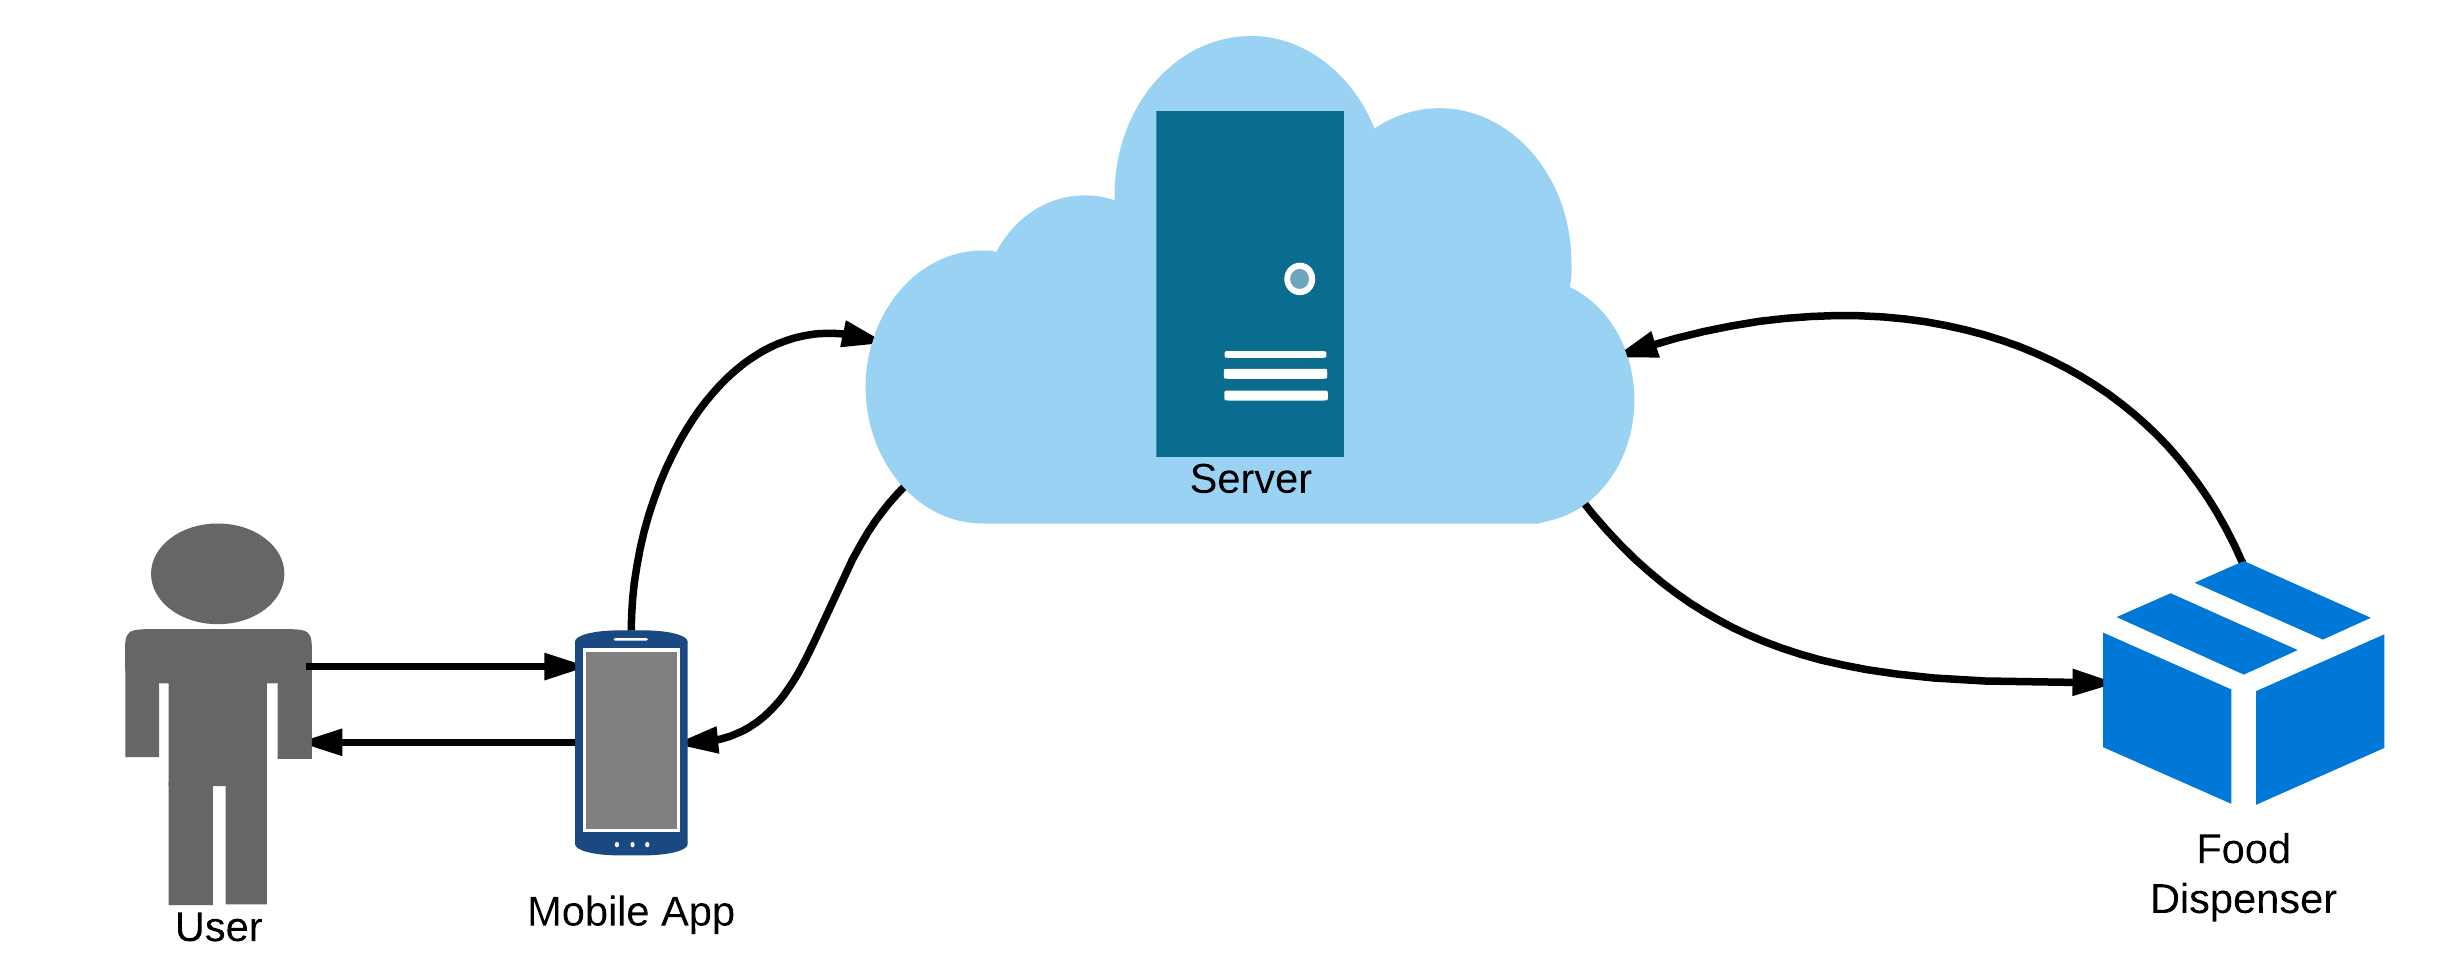
\includegraphics[width=\textwidth]{Figures/GeneralArchitecture}
  \caption{General Architecture}
  \label{fig:GeneralArchitecture}
\end{figure}

Knowing the facts all ready described on the problem definition, we designed a smart food dispenser for dogs capable of being programmed using an mobile application and a web application. Figure \ref{fig:GeneralArchitecture} shows the general architecture of the system. The user uses a mobile or web application to set the dog feeding hours and the time period that the dog will have access to the food if and only if the proximity sensor detects the name tag that the dog wears. After the period conclude, the dispenser will report the amount of food left by the dog if any, and the status of it (temperature and humidity) for quality control.

In order to protect the food and in case of the user owning more than one dog, our smart tag for a dog collar, communicates with the dispenser using Radio Frequency IDentification (RFID) technology. This smart tag allows the dispenser to identify the correct dog that has permission to ingest the food. Also, this feature allows the dispenser to protect the food if the dogs is not near the plate when the meal time comes from rodents and other contaminants already mentioned.

The system will include a battery backup system to allow  proper functioning of the dispenser if the energy coming from the energy provider is interrupted. We will have a server that will contain the databases and serve as the middle man between the dispensers and the users mobile applications.

\subsection{Contributions}

The most remarkable contribution of this design is the huge capability of protect the food by storing the plate inside the dispenser. Thus the only way that the food get exposed is when it gets dispatched for the dog, this means that the programmed hour has arrived and the dog is near. This solution and the feature of controlling the portion size, time of eating and period are good tools for people that owns dogs and don't have enough time to attend their pet, have really busy lives, or are owners that several dogs.

Is important to mention that the reason of the interest on designing this solution came from people having the problems described and more related ones that can be added as future work. Thus dogs owners can have more control of their dogs care and feel more close with them.

Also, based on the research, this dispenser can help decrease the dogs mortality by poisoned food, help prevent obesity, and control the dogs that have bad eating habits by controlling the portions and eating hours.
\newpage

\subsection{Projected Activities}

\begin{figure*}[!htb]
  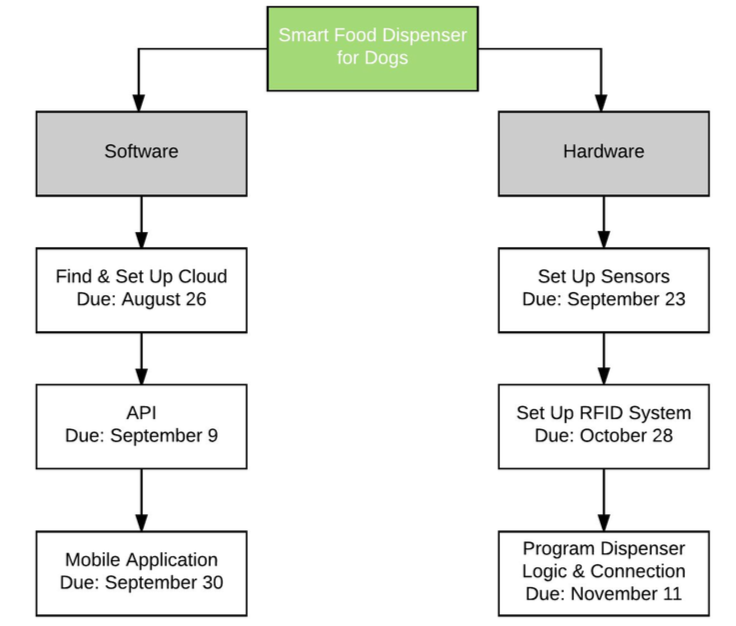
\includegraphics[width=\textwidth]{Figures/ProjectedActivities}
  \caption{Projected Activities}
  \label{fig:ProjectedActivities}
\end{figure*}

\newpage

\subsection{Report Organization}

This report contains all the information related to the design and development process of the dispenser. The information of the technologies where selected to use are described and explained on the Related Word section. The complete description of the system architecture and components selected to work on the plate are included on the System Description Section. Finally, in the Summary section we concluded all the information and provide a conclusion and future work.

% ----------------------------------------------------- Related Work -------------------------------------------------------------

\section{Related Work}

This section will explain every old and new technology used for Capstone 1 and 2 to give the reader some perspective and reasons of why we changed the technology.

\subsection{Bluetooth Low Energy}

Bluetooth Low Energy (BLE) is a wireless personal area network technology used for transmitting data over short distances\cite{IBeacon.com2016}. As the name implies, it's designed for low energy consumption. The main purpose of BLE is for advertisements applications. The three main differences about BLE and Classic Bluetooth are:

\begin{itemize}
 \item Power Consumption: BLE power consumption is very low. The battery can last up to 3 years on a single coin cell battery. This is ideal for some applications where you only need to advertise a device location.
 \item Cost: BLE is 60-80\% cheaper than traditional Bluetooth.
 \item Application: BLE is ideal for simple applications requiring small periodic data transfers. Classic Bluetooth is preferred for more complex applications requiring consistent communication and more data throughput.
\end{itemize}

\subsection{Beacons}

Beacons are one-way transmitters that are used to mark important places and objects\cite{Google2016}. Typically, a beacon is visible to a user's device from a range of a few meters, allowing for highly context-sensitive use cases. These devices are a small low-cost piece of hardware, that use battery friendly Bluetooth Low Energy connections to transmit messages or prompts directly to a smart phone or tablet. Some of the most use cases scenarios are:

\begin{itemize}
  \item Marketing
  \item Place Tips
  \item Indoor location tracking
\end{itemize}

Figure \ref{fig:BeaconCommunication} shows hows a beacon scenario. There are different standards of beacons available. These specifications defines the format of the advertisement message that BLE proximity beacons broadcast. Some of the most famous beacons standards are:

\begin{itemize}
  \item iBeacon: Apple's own protocol specification
  \item Eddystone: Google open source protocol specification
  \item AltBeacon: Emerging open source protocol to compete with iBeacon from Radius Networks
\end{itemize}


\begin{figure*}[!htb]
  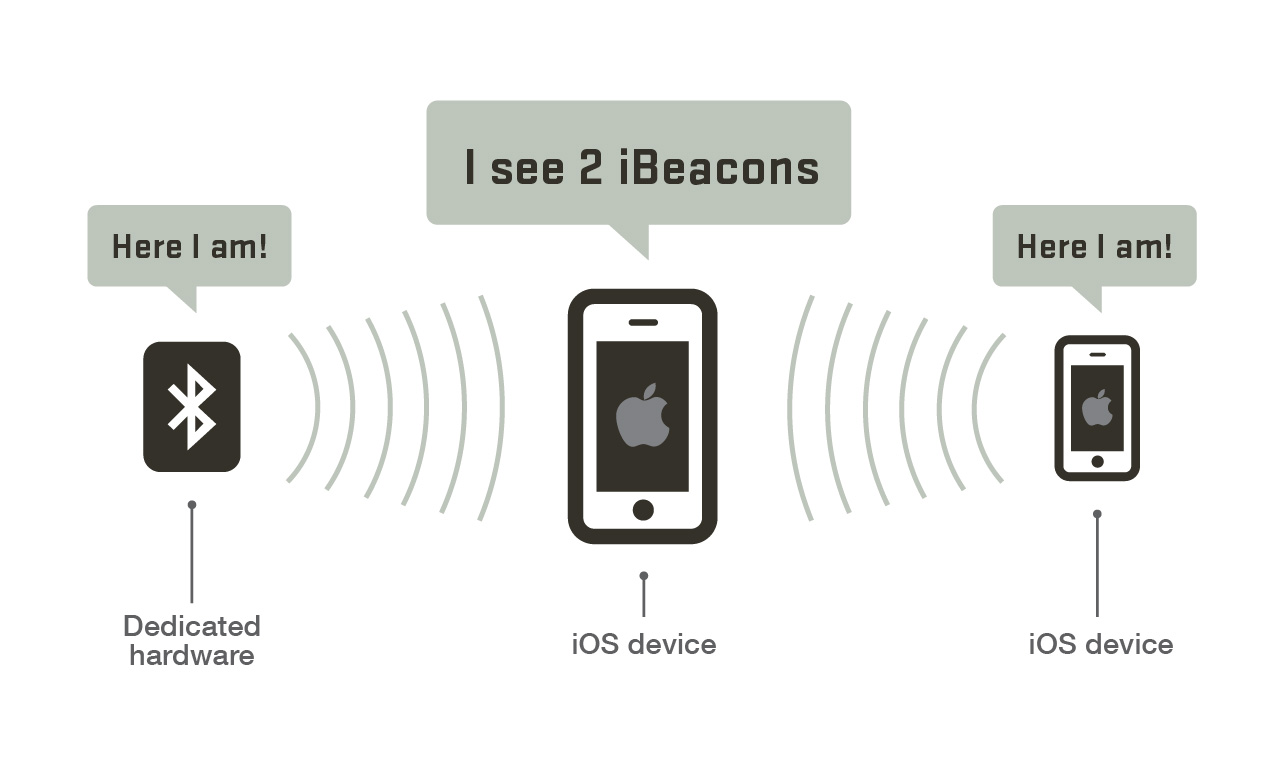
\includegraphics[width=\textwidth]{Figures/BeaconCommunication}
  \caption{Beacon Communication using Bluetooth Low Energy}
  \label{fig:BeaconCommunication}
\end{figure*}


\subsection{Estimotes}

Estimote Beacons an Stickers are small wireless sensors that can attach to any location or object. They broadcast tiny radio signals which a smartphone can receive and interpret, unlocking micro-location and contextual awareness\cite{Estimote2016}. Estimote offers a SDK so that applications can understand their proximity to nearby locations and objects, recognizing their type, ownership, approximate location, temperature and motion. This data can be used to build a new generation of magical mobile applications to connect the real world to a smart device. Estimote Beacons are certified Apple iBeacon compatible as well as support Eddystone. In this project we are using Estimote Beacon Sticker as a dog smart name tag.

\subsection{Socket.IO}

Socket.IO enables real-time bidirectional event-based communication\cite{Rauch2014}. It works on every platform, browser or device, focusing equally on reliability and speed. Also, it simplifies the WebSocket API and unifies the APIs of its fallback transports. Some of the main features that Socket.IO includes are:

\begin{itemize}
  \item Uses HTTP
  \item Bi-directional communication
  \item Can declare what transports to use and the priority of the fallback
  \item Include WebSocket typical connect and disconnect events.
  \item It uses multiplexing
  \item Multiplexing enables namespaces
  \item Scalable by enabling multiple nodes
\end{itemize}


Fallback transports that Socket.IO includes\cite{Kelleher2014}:

\begin{itemize}
  \item WebSocket
  \item Flash Socket
  \item AJAX long-polling
  \item AJAX multi part streaming
  \item IFrame
  \item JSONP polling
\end{itemize}

\subsection{RedBear Duo}

The RedBear Duo is a thumb-size development board designed to simplify the process of building Internet of Things (IoT) products. It provides Wi-Fi, BLE and a powerful Cloud backend, all in a compact form factor that makes it ideal for prototyping, a finished product, and everything in between\cite{Labs2016}.

This microcontroller is cloud ready thanks to a partnership with Particle. A developer can push any changes and data via Cloud right from the start. This is helpful in the development phase and distribution phase because we can update all the microcontrollers at the same time remotely.



% ------------------------------------------ System Description ----------------------------------------------
\section{System Description}

There are many ways to attack the explained problem. The solution has to tackle the following main problems:

\begin{itemize}
  \item Program feeding schedules
  \item Control portion sizes
  \item Send reports to user about how much food is left
  \item Monitor food freshness
  \item Aware of dog presence
\end{itemize}

These problems must be solved with usable and mobile-first as a priority. Having this in mind, there are some characteristics that are very important. Because we are working with dogs, safety is a very important aspect of the project. We must design with safety in mind so that the life of the animal is out of danger. Also, the ease of use, not just for the dog's owner, also for the dog itself is very important. In the decision matrices, from the appendix, we can see how the decisions of the design were taken with this characteristics in mind. From table \ref{tabl:DecLegend}-\ref{tabl:DecDatabase} is shown all the decision matrices for the project.

There are some components that were change due to improvements that needed to be done on the design on the dispenser. The most significant change is the micro-controller. Because of how economical it's, the low power consumption and other features (described on the TABLES) we changed to the Red Beard Duo. Keeping in mid the safety of the dog we decided to change the technology used on the proximity sensor (bluetooth low energy), since it requires the emitter and the receiver to be energized, meaning the collar needs a battery. In order to avoid ingestion from the dog with the collar, this technology was change to RFID (Radio-Frequency IDentification).

The load cell was also changed to the YZC-133 due to the preciseness of this one. The TAL201 could do reading up to 22.0462 pounds (10 Kg) and have and be really precise on readings over 11.0231 pounds, but it could not be so accurate at low loads. We though in this problem keeping in mind the most common amount of food served to dogs. In other hand, the YZC-133 can read 6.6138 pounds (3 Kg) meaning that on low readings like 0.5 pounds we can have good readings. Another reason for the change of load cell is the supply voltages of both, the TAL201 works from 5 to 10 Volts and the YZC-133 works at 5 V.

Like we can see in the decision matrices, we have several categories of components. Here is a summary of the actual components that we choose according to the tables. Components:

\begin{itemize}
  \item Controller: Red Bear Duo
  \item Proximity: RFID 125KHz
  \item Temperature and Humidity Sensors: DHT11
  \item Distance Sensor: HR SR04
  \item Load Cell: Straight Bar (YZC-133)
  \item Connection: Red Bear WiFi Module
  \item Server: Node.js
  \item Database: PostgreSQL
\end{itemize}

The decisions were made for all categories. However, we will see in the next subsection how we combine the controller, proximity and connection in just one component thanks to the capabilities of the Red Bear Duo.

\subsection{Food Dispenser}

\begin{figure*}[!htb]
  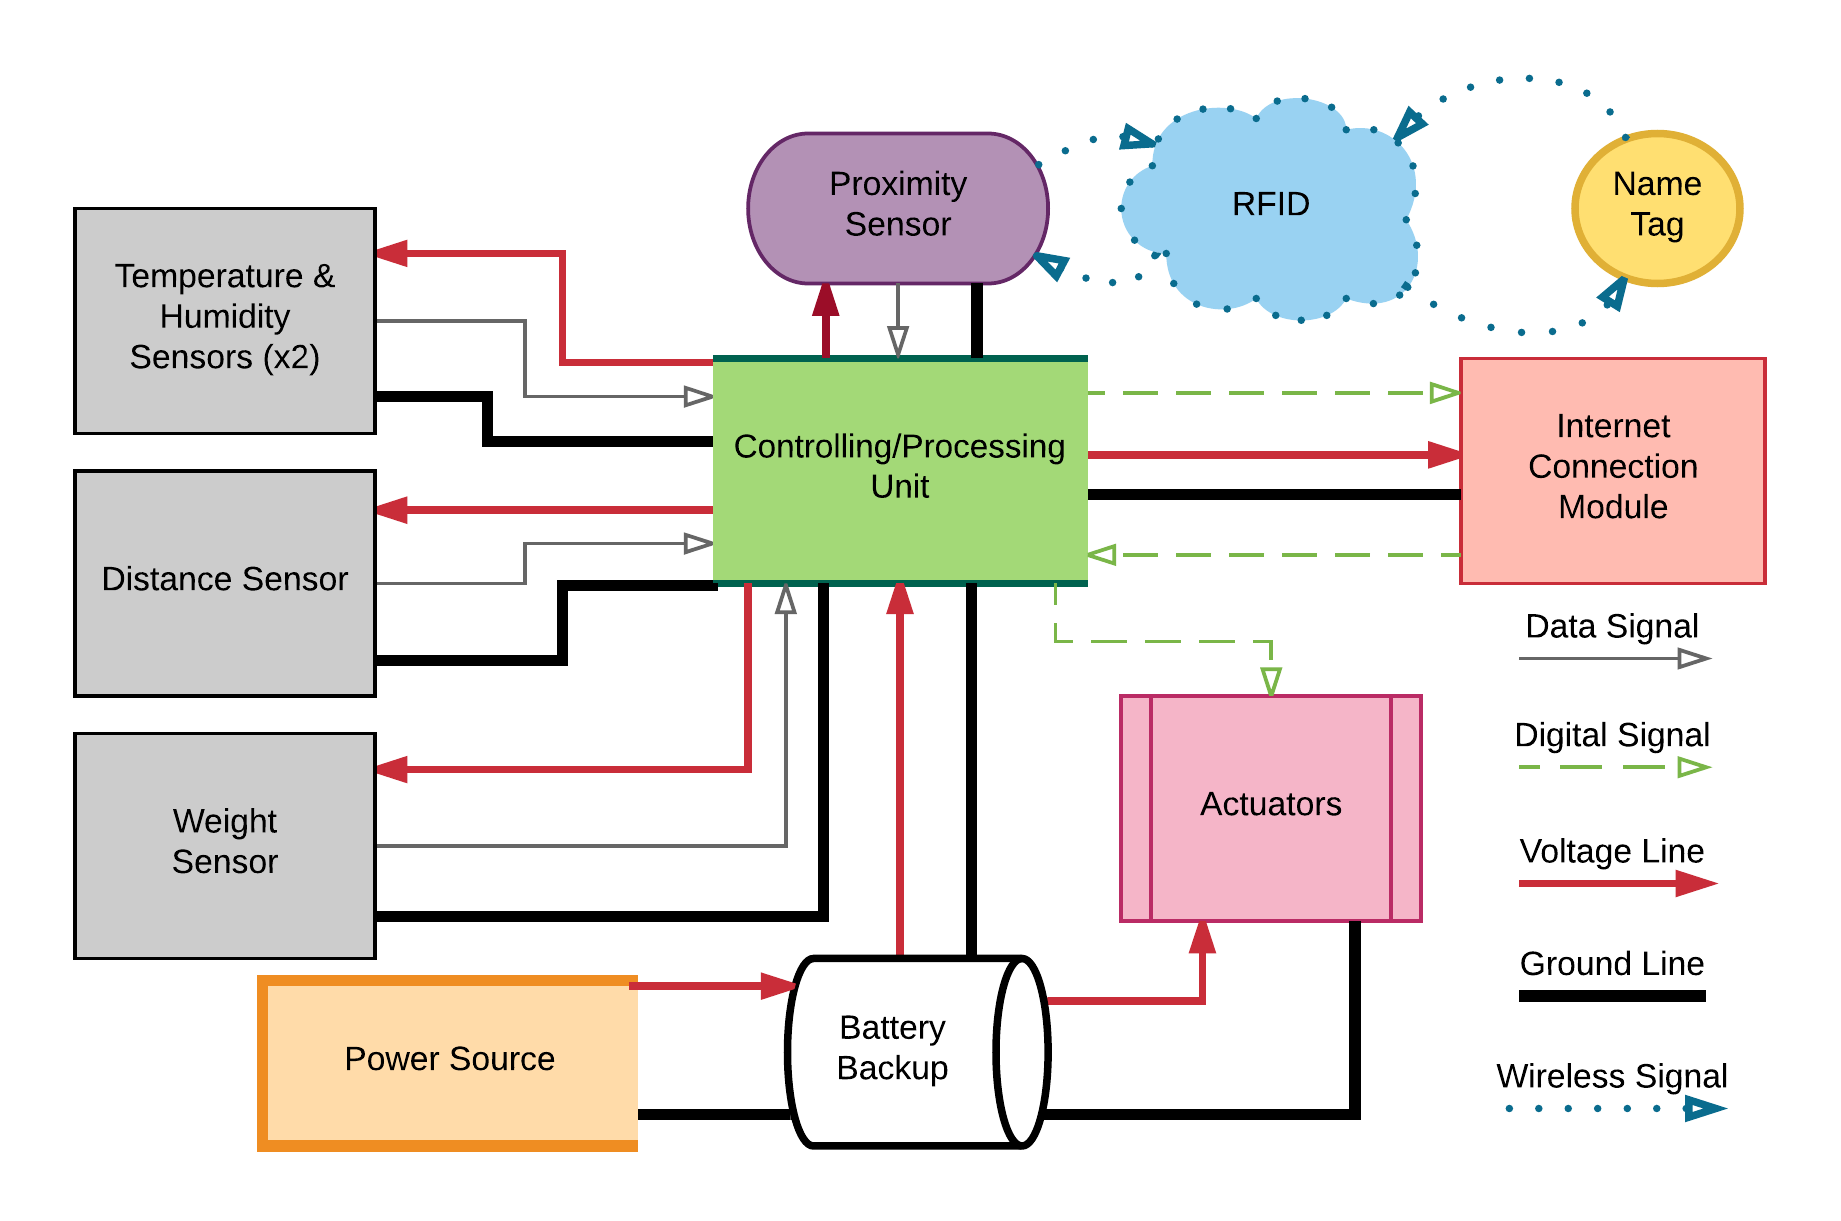
\includegraphics[width=\textwidth]{Figures/ArchitectureDispenser}
  \caption{Dispenser Architecture}
  \label{fig:ArchDispenser}
\end{figure*}

\subsubsection{Controller/Connection Unit}

The Controller/Processing Unit is the component or that will control every process the may be required. This basically is the brain of the dispenser. In table \ref{tabl:DecController} we can see that the Red Bear Duo won in the decision process.

We choose the Red Bear Duo because of all the features that includes this micro-controller in a small package for its economic price of \$25. We are going to use the built in Wi-Fi  as our Connection. This controlling unit will be in charge of controlling:

\begin{itemize}
  % \item Being aware of dog presence using the BLE
  \item Read temperature and humidity from both, food bowl and food container
  \item Read how much weight is in both the food bowl and the food container
  \item Connect to the Internet
  \item Send data collected to the server
\end{itemize}

The Connection Unit of our system is solved using the built in WiFi module that the Red Bear Duo has. We are going to use this module to connect to the server via Internet using our own rest http API.

\section{Proximity} % (fold)
\label{sec:proximity}

As for the Proximity Unit, we are using an RFID tag\cite{K2014} as the smart name tag that the dispenser will detect by using an RFID module. If the smart name tag is 1.37 inches nearby and is time to eat, according to the schedule that the owner programed, the dispenser will open the bowl of food. As soon as the dog is not nearby or the time of eating is due, the bowl will close the bowl of food. The smart name tag has an technically infinite life time since it is a passive element and does not need any power source to work.

The RFI module works at 125KHz and it sends a radio frequency signal to the tag and the tag bounces back the signal containing the ID of the tag. The work distance is currently really near to the module due that this design is focus on the proof of concept. On the future we plan to change this technology or improve the performance of it.

% section proximity (end)


\subsubsection{Sensors}

The design includes three types of sensors to measure important characteristics of the food. We included temperature and humidity sensors to measure food freshness and a weight sensor to know how much food is left on both the food bowl and food container.

For the temperature and humidity sensor, as table \ref{tabl:DecSensors} shows, we selected the DHT11 sensor. The DHT11 sensor includes both temperature and humidity sensor in a single body. Also, the output of the module is digital. This is perfect as the Red Bear Duo do not include any analog input.

The system should report how the dog is eating referring to his habits. This is possibly in our design thanks to the weight sensor. The dispenser will measure how much food is left in the bowl. With the collected data, the system should report to the user mobile application if the dog did eat or not. Using this information, we can generate weekly reports about the eating habits of the animal. This way, the dog's owner can know how his/her dog is eating and can monitor the dog's health.

In this design we included one more sensor, the HC SR04. This sensor will is used to measure the amount of food inside the canister by reading the distance between the food and the sensor. In this manner we can create alarms based on food amount status.

\subsubsection{Battery Backup}

To calculate the system power consumption we used the Red Bear Duo and DC Motors peak Voltages and Currents. This way we can know the how much energy we need to supply to the system in the case it needs it. Also, this is helpful information to select the best miliAmps per Hour battery for the Battery backup that the system will have.

The sensors power will be provided from the Red Bear and this values are assumed by the energy consumed from it. The Red Bear peak voltage and amperage are 3.3V and 1A, making it to dispel \(P = IV\) around 3.3 Watts of electric energy. The same way, the DC motors selected for this project works with a peak voltage and current of 6V and 1.7 Amps with load, meaning a that booth will consume 20.4 Watts on their peaks values.

Knowing that additive in any configuration of resistive circuit, the total peak power of the circuit is approximately 11 Watts. The system works with 6V and the for calculate the current that the circuits needs for its peak values the same formula of power\cite{AllAboutCircuits} has been used as follows:

\begin{itemize}
  \item \(P = IV\)
  \item \(I = P/V\)
  \item \(I = 11W/6V\)
  \item \(I = 1.83A\)
\end{itemize}

From doing some research for choosing the correct battery for backup, the type selected is a Li-Ion one for various reasons. Some of them are:

\begin{enumerate}
  \item Usable Capacity

  \begin{itemize}
    \item Unlike with lead acid batteries, it is considered practical to regularly use 85\% or more of the rated capacity of a lithium battery bank, and occasionally more.
  \end{itemize}

  \item Fast \& Efficient Charging
  \begin{itemize}
    \item Lithium-ion batteries can be “fast” charged to 100\% of capacity. Unlike with lead acid, there is no need for an absorption phase to get the final 20\% stored.
  \end{itemize}
\end{enumerate}

To meet peak values system we need a battery of about 1.2 Amps per hour to keep the circuit in operation for two hours at peak values. these values can be improved by working more efficiently the circuit is to be implemented.

The battery selected is the Tenergy Li-Ion 18650 Rechargeable Battery Pack w/ ca=harge controller PCB. The technical specs of the battery are

\begin{itemize}
  \item Type: Pack
  \item Chemistry: Li-ion
  \item Nominal Voltage (V): 7.4
  \item Capacity (mAh): 4400
  \item Max Continuous Discharge Current: 5.0A
  \item Battery Charging Current:
  \begin{itemize}
    \item Standard: 0.9A
    \item Rapid: 2A
  \end{itemize}
  \item PCB/Pack Protection:
  \begin{itemize}
    \item Overcharge Protection: $>$ 8.4V
    \item Over-discharge Protection: $<$ 6.0V
    \item For Detailed PCB Info: (click here)
    \item Over Current Cutoff (A): 11 $\pm$ 3A
  \end{itemize}
\end{itemize}

\subsection{Server}

\begin{figure*}[!htb]
  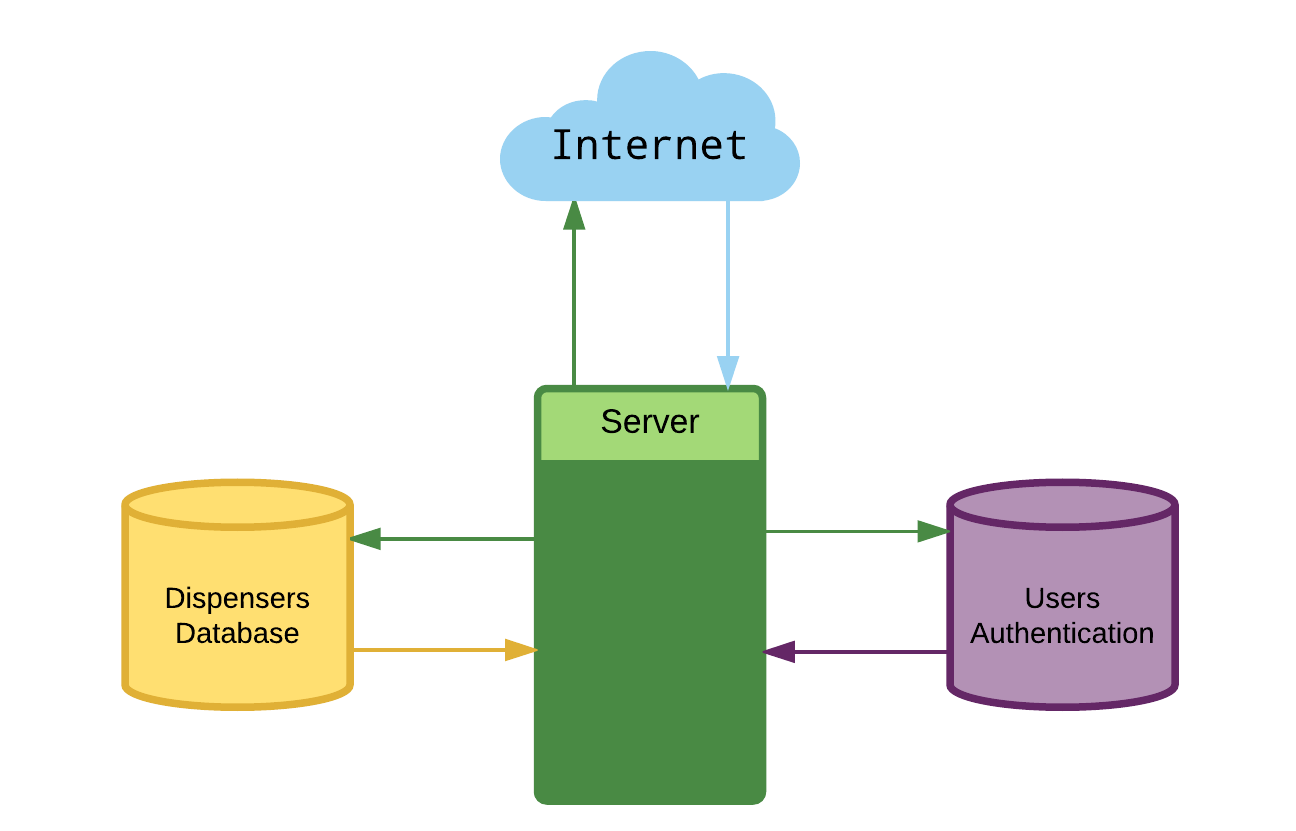
\includegraphics[width=\textwidth]{Figures/ArchitectureServer}
  \caption{Server Architecture}
  \label{fig:ServArchitecture}
\end{figure*}

To be able to connect the dispenser with the mobile application no matter where the user is, we need a server. As we can see in table \ref{tabl:DecServer}, the server is a Node.js server. We selected to develop our server in Node because for its ease of use and support of new technologies like Socket.IO.

Our server will be our intermediate between a dispenser and a user mobile application. It will have 2 databases. One PostgreSQL database with all the information about dispensers, sensors, feeding schedule, data about food temperature and humidity, and a second one hosted in Microsoft Azure cloud Active Directory for security purposes. Figure \ref{fig:EntityRelationship} shows the entity relationship diagram of the database.

\begin{figure*}[!htb]
  \begin{center}
    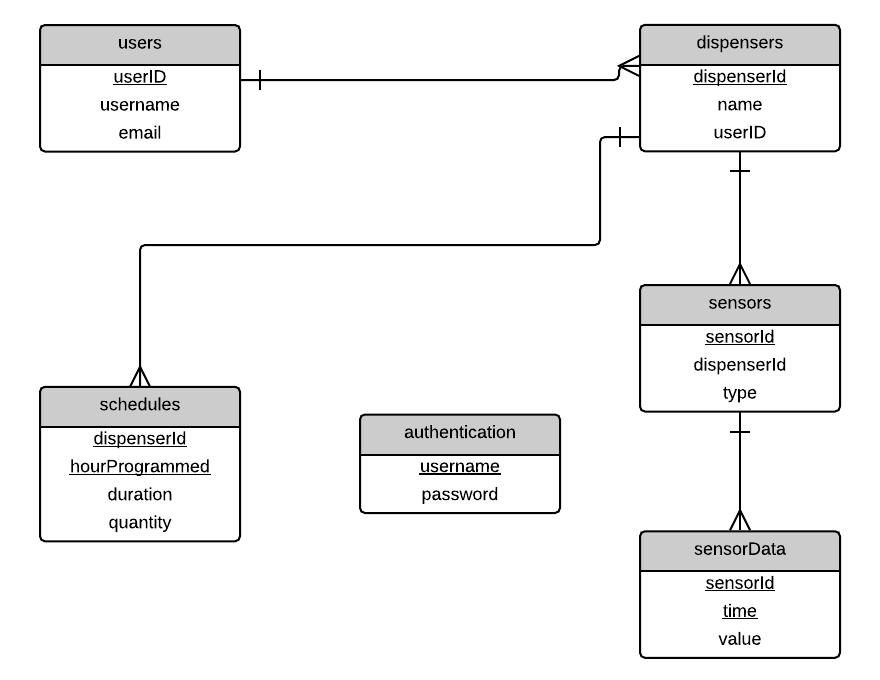
\includegraphics[scale=0.35]{Figures/EntityRelationship}
  \end{center}
  \caption{Entity Relationship Diagram}
  \label{fig:EntityRelationship}
\end{figure*}


\subsection{Mobile Application}

\begin{figure*}[!htb]
  \begin{center}
    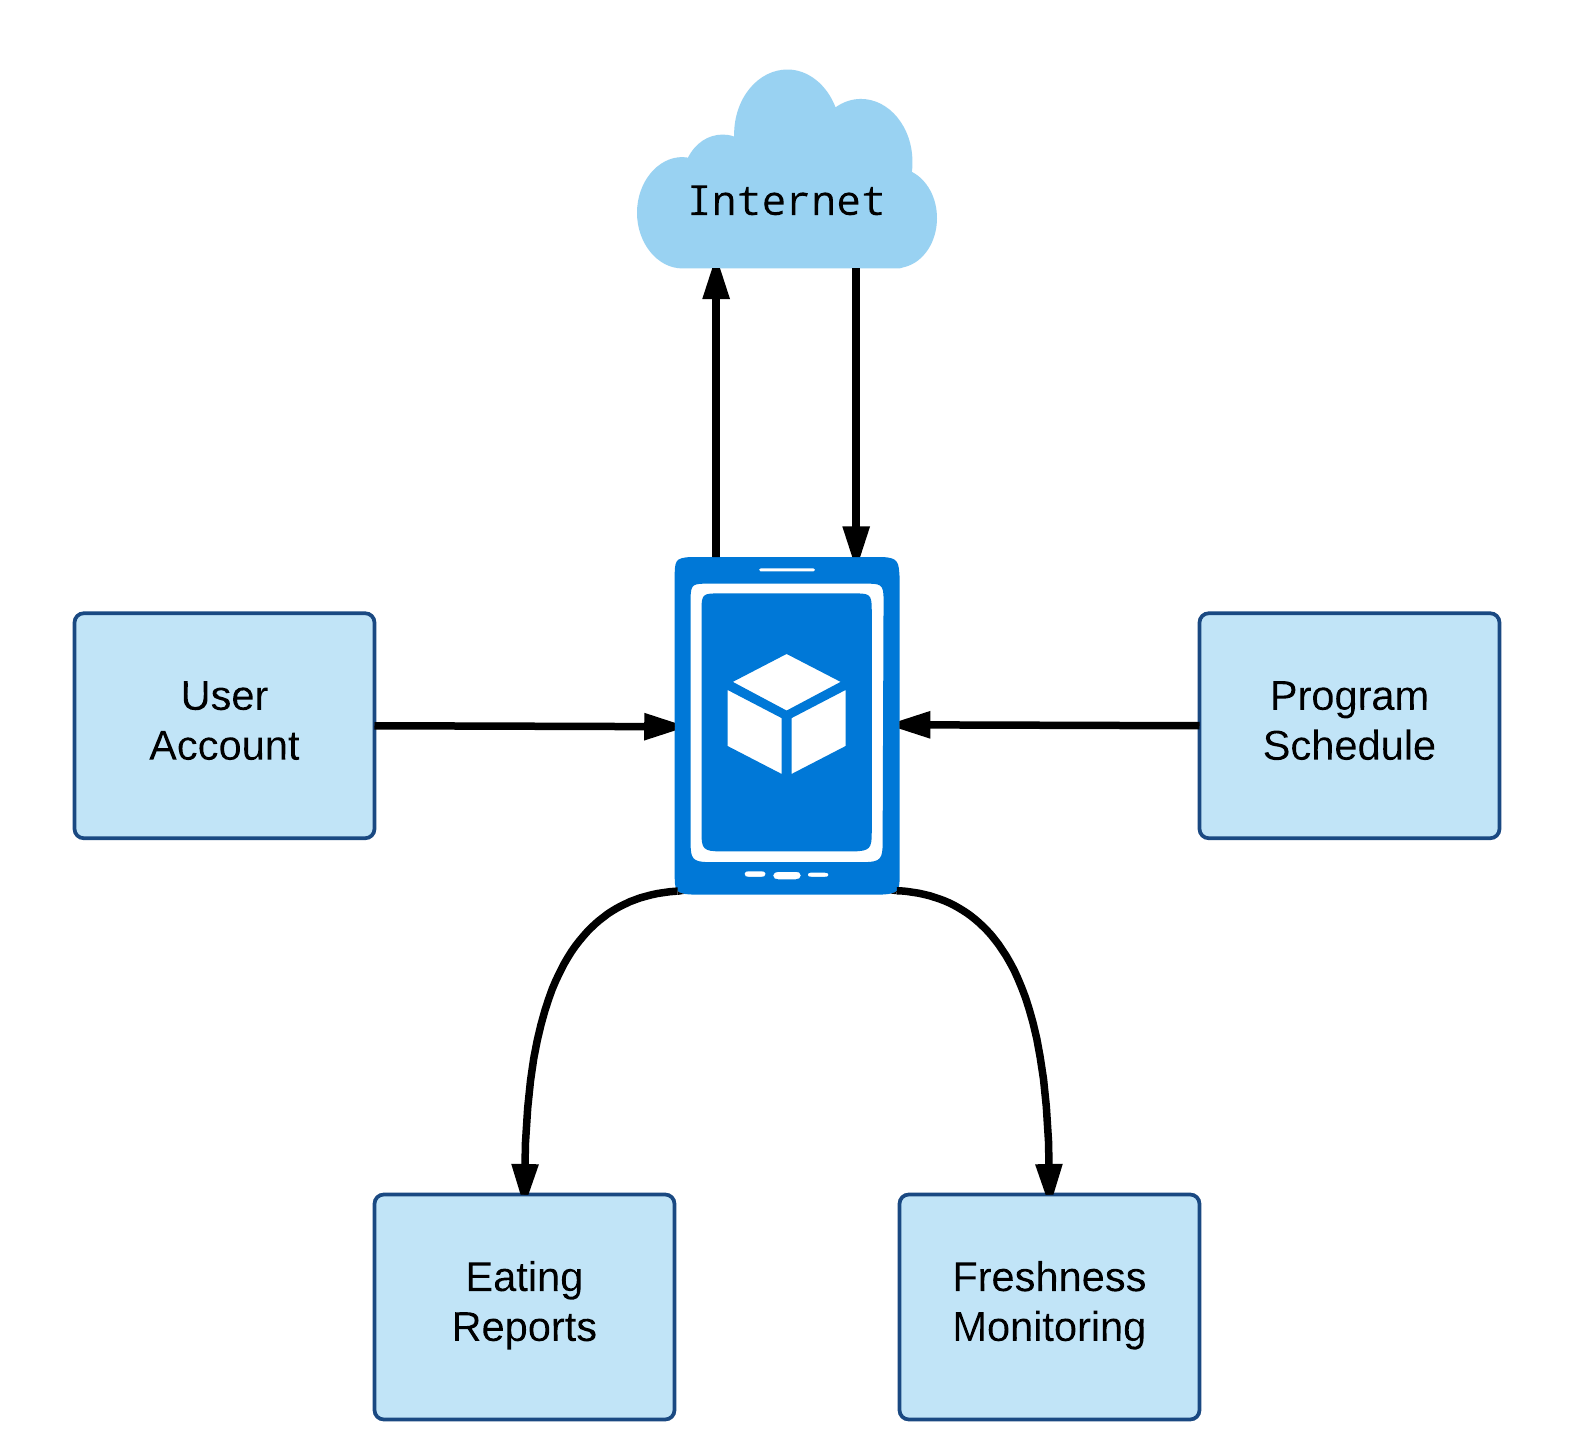
\includegraphics[scale=0.2]{Figures/ArchitectureApplication}
  \end{center}
  \caption{Mobile Application Architecture}
  \label{fig:AppArchitecture}
\end{figure*}

To complete the general architecture as shown in figure \ref{fig:GeneralArchitecture}, we designed an iOS application for the dog's owner. This application will let the user log in into an account, view all user's dispensers, program schedules, view eating reports and monitor food freshness. The application communicates with the server using Socket.IO. The application is divided in three parts. Figure \ref{fig:AppFlowchart} shows the mobile application flowchart with the three parts indicated.

\begin{figure*}[!htb]
  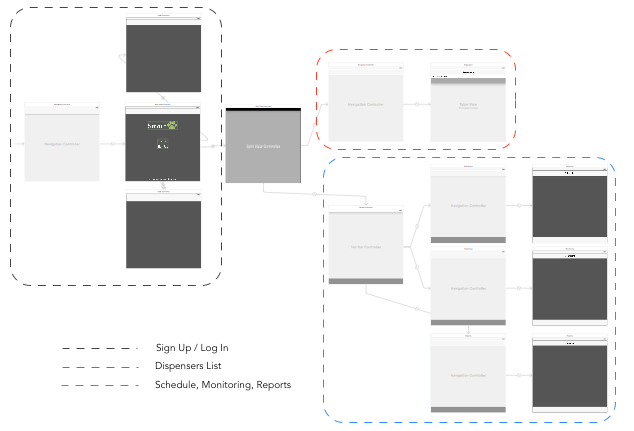
\includegraphics[scale=0.6]{Figures/MobileAppScenes}
  \caption{Mobile Application Flowchart}
  \label{fig:AppFlowchart}
\end{figure*}

The first one is the Sign Up/Log In scenes. This is where the user need to authenticate before having access to the dispensers configurations and main features. The authentication process will use Microsoft Azure Active Directory\cite{Vilcinskas2016}. This service allows the developer to add a simplified authentication process where you can create a custom account or sign up/ log in with a Facebook account.

The next part of the application is the dispensers list. This scenes will allow the user to see all the proper registered dispensers. Additionally to that, the user will have the option to configure a new dispenser. This process will consist of scanning for near dispensers using Bluetooth. After detecting a dispenser, this link will be saved in the server database. During the configuration process, the user will need to configure the  WiFi network of the dispenser. The user will see a list of the available WiFis networks that the dispenser detected, and will have to select one. The user must input the corresponding network password and send it back to the dispenser. After making this configuration, all the communication between the dispenser and the mobile application will be by using the server as the middle man.

The last part of the mobile application consist of the main features. The user will be able to schedule, monitor, and see reports of eating habits of a dog. In the scene of scheduling eating times, the user will need to input from what hour to what hour, the portion size, and if it repeats daily. In the monitor scene, the user will have a table with the data collected from the temperature and humidity sensors. And last, in the report scene the user will see graphics about how the dog is eating and a table with all the collected data from the dispenser.


\section{Conclusions and Future Work}

This report presents a system that solve some of the main problems that dog owners have when feeding their pets. The system uses a Red Bear Duo as the brain of the dispenser and protects the food when a smart name tag is not nearby. This smart name tag uses RFID technology as proximity detection . Also, the dispenser monitor and reports to the user food freshness and dog's eating habits. All this is reported and programmed by using a mobile application. Our system is in the proof of concept stage of development. We were able to:

\begin{itemize}
  \item Program the hour of eat, period of time and food portion.
  \item Serve the programmed food portion the the time programmed
  \item Detect the dog and make the food available if the dog is near
  \item Monitor the food temperature, humidity and quantity in the plate and canister
\end{itemize}

In order to complete the design, we need to work the aesthetics of the dispenser and how the mechanical aspects of the dispenser should work.

For future work, we need to implement the proposed design, consider water integration in the dispenser, and research more if RFID is a more suitable technology for the smart name tag. Also, we should consider if a single dispenser can be used with several dogs.

The most remarkable contribution of this design is the huge capability of protecting the food by retracting the plate inside the dispenser. Is important to mention that the interest on designing this solution came from people having the problems described in the problem definition. We are contributing and simplifying peoples live by empowering them to have control over his/her dog's eating habits.


\section*{Acknowledgment}

Special thanks to Dr. Vergara for supporting this project with his mentorship and guidance.

\newpage
\bibliographystyle{ieeetr}
\bibliography{Referencias}{}

\newpage
\begin{appendix}

  \listoffigures
  \listoftables

  \begin{table}[!htb]
    \begin{center}
      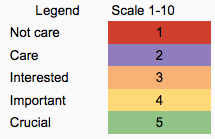
\includegraphics[scale=1]{Figures/DecisionMatrixLegend}
    \end{center}
    \caption{Legend of Decision Matrix}
    \label{tabl:DecLegend}
  \end{table}

  \begin{table*}[!htb]
    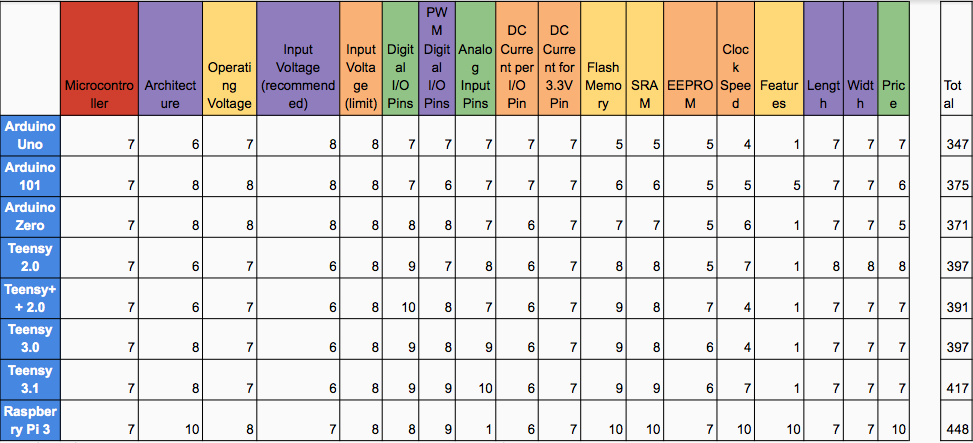
\includegraphics[width=\textwidth]{Figures/DecisionMatrixController}
    \caption{Controller Decision Matrix}
     \label{tabl:DecController}
  \end{table*}

  \begin{table*}[!htb]
    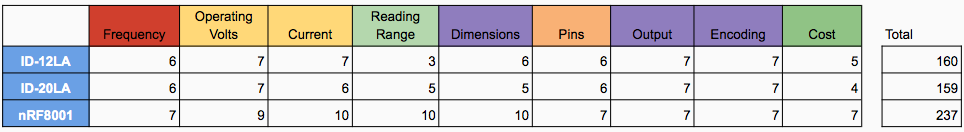
\includegraphics[width=\textwidth]{Figures/DecisionMatrixProximity}
    \caption{Proximity Decision Matrix}
     \label{tabl:DecProximity}
  \end{table*}

  \begin{table*}[!htb]
    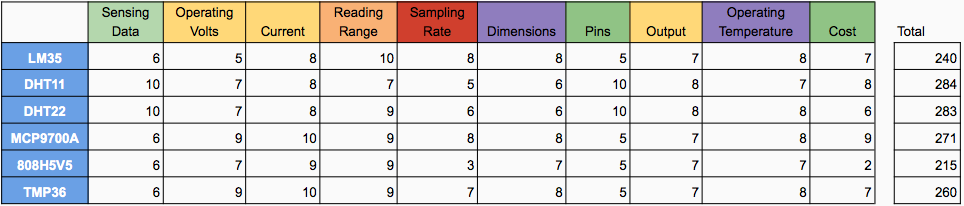
\includegraphics[width=\textwidth]{Figures/DecisionMatrixSensors}
    \caption{Sensors Decision Matrix}
     \label{tabl:DecSensors}
  \end{table*}

  \begin{table*}[!htb]
    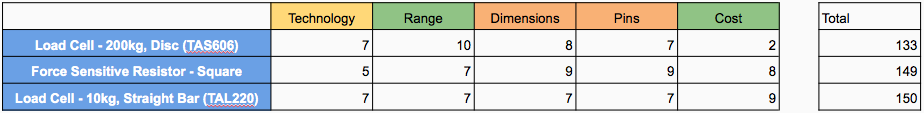
\includegraphics[width=\textwidth]{Figures/DecisionMatrixLoadCell}
    \caption{Load Cell Decision Matrix}
     \label{tabl:DecLoadCell}
  \end{table*}

  \begin{table*}[!htb]
    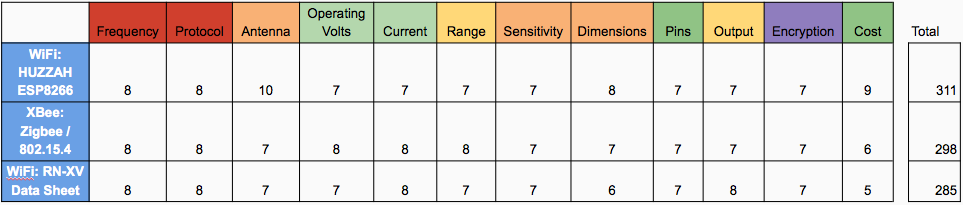
\includegraphics[width=\textwidth]{Figures/DecisionMatrixConnection}
    \caption{Connection Decision Matrix}
     \label{tabl:DecConnection}
  \end{table*}

  \begin{table*}[!htb]
    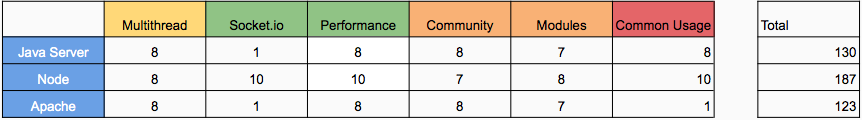
\includegraphics[width=\textwidth]{Figures/DecisionMatrixServer}
    \caption{Server Decision Matrix}
     \label{tabl:DecServer}
  \end{table*}

  \begin{table*}[!htb]
    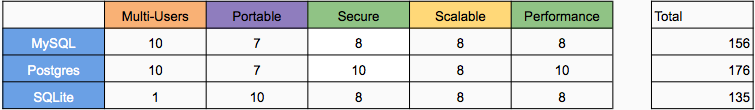
\includegraphics[width=\textwidth]{Figures/DecisionMatrixDatabase}
    \caption{Database Decision Matrix}
     \label{tabl:DecDatabase}
  \end{table*}

\end{appendix}
\newpage





% that's all folks
\end{document}
